\section{System Description}

% describe overall system
As input, our system for retrieving follow-up questions requires: 1) an inadequate bug
report of interest; 2) a corpus of already posed follow-up questions extracted
from GitHub issues, including their corresponding bug reports and answers. As output, our system
produces a ranked list of follow-up questions appropriate to the inadequate bug report.
In this section, we describe our system, including how we create as a input
a large corpus of follow-up questions to recommend, how we select candidate follow-up questions from
this corpus for a specific incomplete bug report, and how we rank these questions in descending order of
their potential utility to the bug report.

\subsection{Selecting a Corpus of Bug Reports}


\begin{figure*}[ht]
\centering
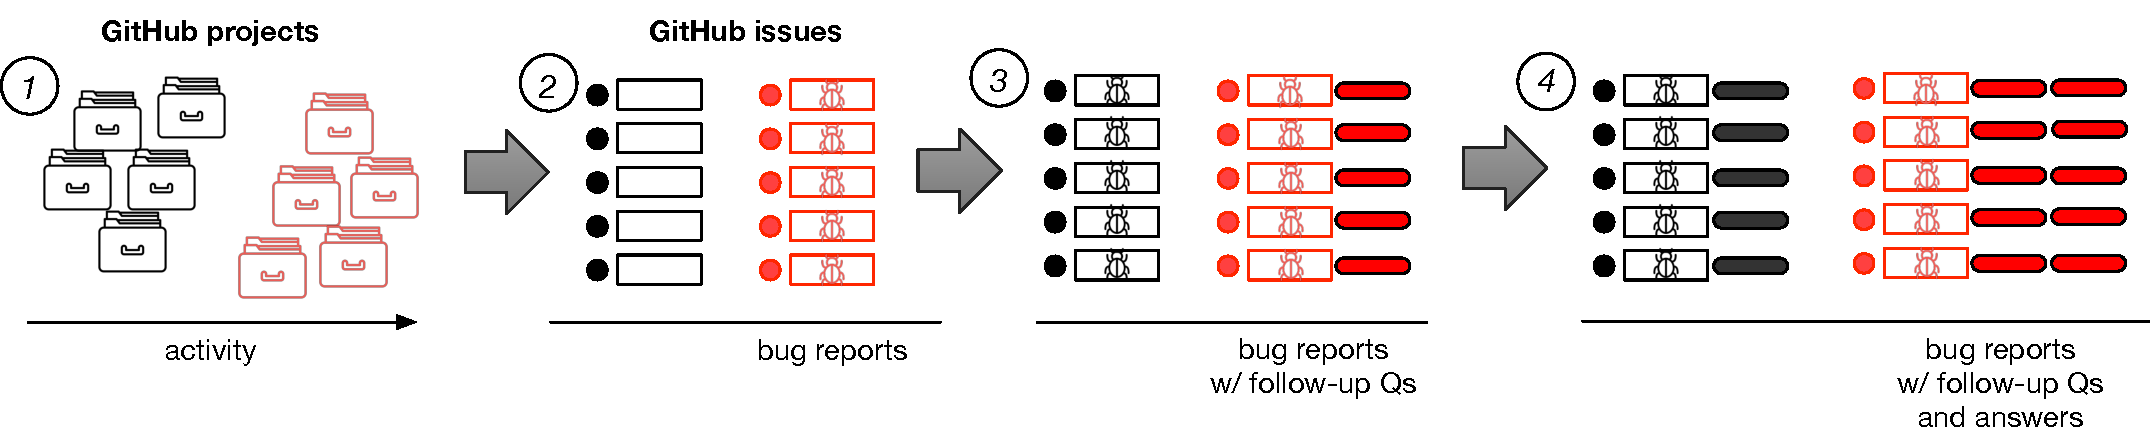
\includegraphics[width=0.99\linewidth]{figures/pipeline.pdf}
\caption{Automatically curating a input corpus for our system follows a sequence of filtering steps, starting with filtering
GitHub repositories to selecting only the issues in these repositories that are bug reports with answered follow-up questions.}
\label{fig:sample_br}
\end{figure*}

% overview of the entire process
Our goal in curating a corpus of bug report-related follow-up questions and their answers
is to find a large, representative and high-quality corpus. Manually curated corpora are of
high quality but they are difficult to scale-up. Automatic curation can easily scale but it
can be affected by significant noise, leading to low data quality, unless care is taken
to filter and sample follow-up questions in a way that noise is mitigated. As corpus size
is an important factor in our system, we opt for an automated approach with numerous filters
to ensure the data is of highest possible quality. With the number of active repositories available
on GitHub providing a very large input domain, we can afford to err on the side of being overly
restrictive in our filtering.
To automatically curate our corpus, we: 1) select GitHub repositories that have high bug reporting activity,
as measured by the number of issues created by non-contributors over some fixed period of time; 2) select issues in those bug repositories that contain rapidly asked and succinct follow-up questions contained in GitHub issue comments; 3) locate
answers to the follow-up questions encoded as either comments or as edits to the
original bug report.

In more detail, we used the following sequence of steps to curate the corpus. The highlights of the corpus curation process are also illustrated in Figure~\ref{fig:sample_br}.
\begin{enumerate}
\item We scraped a set of public GitHub repositories with a high rate of
non-contributor created issues, where a non-contributor is a GitHub user that has never
committed any code in the specific repository. Repositories with these characteristics form
the target population of software projects that are more likely to use our technique. In order
to somewhat constrain  the amount of repositories, we focused on longer-running projects,
specifically, created between 2008-2014, and recently active with new issues created in the repository after Jan 1, 2019.
\item For each of these repositories, in their descending order of activity as defined in the previous step,
we selected issues in their GitHub issue tracker that are labeled as ``bug", ``crash", ``fix", ``defect" or unlabeled. Our goal for this step was
to avoid feature requests and focus on bug reports. We observed that issue labels were not used consistently enough
in projects, which is why we opted to include unlabeled issues. Since we are interested in incomplete bug reports, we select bug reports that do not contain Observable Behavior, Expected Behavior or Steps to Reproduce. While focusing on incompleteness in one of these categories is possible, for simplicity, we chose bug reports that lacked all three.
\item We further selected only issues that contain follow-up questions in one of the issue comments.  We identified follow-up questions as GitHub comments containing only questions, identified by both starting with an interrogative word and ending with a question mark. In order to ensure we selected follow-up questions and not just
any questions, we constrained our selection based on time and comment sequence. That is, the comment containing the follow-up question must have been posted within 60 days of the issue creation date and must have occurred as the comment immediately following the post. We also ignored follow-up posts by the issue author by ensuring that the comment was authored by a different user from the author of the issue.
\item The set of issues and candidate follow-up questions from the previous step were further filtered to
retain issues and follow-up questions where an answer was provided. A key heuristic we used for recognizing an answer was that it was authored
by the original issue creator and occurred as the the next sequential comment
to the follow-up question. We also searched for answers that were encoded as edits to the original issue text by the author, which occurred after the follow-up question was posted and were limited to add at least 4 additional words to the original text in order to avoid minor spelling or grammar modifications.
\end{enumerate}

 We stopped the collection process when we gathered a dataset of 25K GitHub issues, which we deemed to be sufficient for our purpose. Each data point in our dataset is a triple of
issue, follow-up question, and answer. Together, the 25K triples form the primary corpus we used to
retrieve and rank follow-up questions for a given inadequate bug report.


\subsection{Selecting Candidate Follow-Up Questions}

Selecting a set of most likely candidate follow-up questions for a specific incomplete bug report of interest from the corpus
of 25K triples (bug reports, follow-up questions and their answers) can be formulated as an information retrieval
problem. That is, as a query we can use the text of the incomplete bug report. We can represent the corpus
as an inverted index of the bug report text (e.g., using Lucene), and use tf*idf as the
ranking mechanism. In this way, we retrieve a set of 10 candidate follow-up questions for each incomplete bug report
of interest, where these 10 candidates have the most similar bug report text to the bug report of index.

More specifically, we create a Lucene index of the corpus of bug reports by following this set of steps:
\begin{itemize}
\item {\em Filtering.} Removing code or stack traces from bug reports in our index allows
for more accurate matching. GitHub issues use markdown so we remove all text surrounded
by triple-quotes as this is typically how source code and stack traces are encoded. We also
remove quoted text (i.e., lines that start with the greater than symbol) as these typically
refer to some external information, which, again, is often stack traces, code, or project documentation.
\item {\em Tokenization.} We perform standard tokenization used in software engineering applications
of information retrieval~\cite{marcus2004information,shepherd2012sando}. We tokenize on white space, remove
punctuation (except for horizontal dashes)
and split on camel case and dashes, while also keeping the original unsplit tokens.
\item {\em Indexing.} We use Lucene's standard configuration to index the title and the body in separate fields,
in order to ensure better quality matches, especially when the bug report body has a lot of text. In order to provide
more context, we extract the tags that the bug report is labeled with (e.g., {\em fix-later, critical}) and the tags the
GitHub repository is tagged with (e.g., {\em java, linux, web-server}). The former provides specifics on the issue while the
latter usually denotes technologies or the project uses or broad categories it belongs to.
\end{itemize}

To create a query out of the incomplete bug report, we tokenize the its title and body
using the equivalent process to the one we performed on the bug reports in the corpus.
While obtaining a ranked list of follow-up questions from Lucene, we obtain and list of 10
triples and ignore the ranking. In the following section, we describe a customized ranking, which
takes more factors into account when choosing which follow-up question to pose to the inadequate
bug report.


\subsection{Ranking the Candidate Follow-Up Questions}\label{sec:ranking}

To rank the set of candidate follow-up questions we reformulate and apply towards bug reporting
the notion of the Expected Value of Perfect Information (EVPI), initially proposed as a means to
rank follow-up quesitons by Rao et al.~\cite{rao-daume-iii-2018-learning}. To evaluate a follow-up question, EVPI suggests
using the (expected) value of its answer, i.e., for an
incomplete bug report, EVPI estimates the value of the information provided by the answer to the
follow-up question. The higher the EVPI the higher we rank a follow-up question from the candidate
set.

Given an inadequate bug report of interest, $br$, we express the EVPI of a specific follow-up question $q_{i}$ from our candidate set
as the product of: 1) the compatibility of a specific follow up question to the bug report, i.e.,
the probability of a specific question and answer pair occurring for that bug report, $P(q_{i}+a_{i}|br)$, and 2) the utility of that question, $U(q_{i})$.

$$EVPI(q_{i}|br) = P(q_{i}+a_{i}|br) * U(q_{i})$$

The utility of a question is further expressed in terms of the average quality of the answers it has received, i.e.,

$$U(q_{i}) = \frac{1}{|A|} * \sum_{a \in A}^{} \frac{|OB(a)|+|EB(a)|+|S2R(a)|}{|a|}$$

\noindent
,where $A$ is the set of answers $q_{i}$ has received in the corpus, $a$ is one of those answers, and
$OB(a)$, $EB(a)$ and $S2R(a)$ are the sentences describing Observable Behavior (OB), Expected Behavior (EB), or
Steps to Reproduce (S2R) found in the answer. We use the $|\cdot|$ operator to denote the cardinality of a set.
The idea of this metric is that questions whose set of answers have a high proportion
of OB,EB, or S2R of a bug report have higher utility than do questions whose answers do not contribute much in
terms of this information.

To compute the probability of a follow-up question occurring for a given bug report, $P(q_{i}+a_{i}|br)$, we use a neural
network approximation, using a deep NN consisting of 3 layers. As the first layer, in order to introduce semantics, we encode
the bug report text with GloVe word embeddings that we pre-trained on the entirety of Stack Overflow. As the second layer, in order to capture the word sequence, we train a LSTM and compute an average across the hidden LSTM layer. As the third and final layer we use a dense neural network consisting of 4 inter-connected layers. The output is the concatenation of the average word embeddings of $q_{i}$ and $a_{i}$. We train this neural architecture using the actually posed follow-up questions and answers as positive labeled examples and the remaining question-answer pairs in the candidate set as negatively labeled, computing the average GloVe word embeddings for each of the labeled examples. We use cosine embedding loss and weight balancing to manage the resulting class imbalance as the negative examples significantly outnumber the positive ones.

To compute the utility of the follow-up question, $U(q_{i})$, we leverage the pattern based
identification of the constituent pieces of a bug report (OB,EB and S2R) created by Chaparro et al.~\cite{chaparro17detecting}
We implement 5 of the most common and most productive patterns for each of OB,EB and S2R, as described by
the authors. Each of the total 15 patterns we implemented rely on predefined sets of keywords and part-of-speech tagging to ensure high
precision. In order to compute the average utility of the answers for a particular question in the corpus, we rely on Lucene to provide
matching between questions and we reserve 10 of the most similar question variants for each queried follow-up question.


%
% p(a_i|q_i,p_i) is estimated via a 5-layer feed-forward NN.
%
% U(p+a) = softmax(d_OB+d_EB+dS2R), where dOB = OBa_i - OBp, and similarly dEB and dS2R
%
% OB_x is the number of OB sentences in document x, as defined by Chaparro et al.
